\section{Introduction}
% 1. Describe the Current Situtation
% Functions as a starting point and a common basis. Therefore it primarily contains recognizable and agreed points.
% 2. What is the complication, challenge identified
% Spells the reason for acting now. It contains threats / opportunities and the hurdles that need to be overcome.
\todo{add something even more general here: e.g. increase human wellbeing by XY}
Advances in hardware that augment a user's physical actions have reignited dreams of overcoming human limitations, recovering lost abilities as well as simplifying skill acquisition~\citep{Kasahara2019-sk, Goto2020-mw}. There are two main technologies to physically augment users' actions: Through the use of mechanical actuators, i.e. exoskeletons, a user's body can be moved by applying forces to the extremities, for example by pulling on the fingertips. Another technology makes the user's extremities move by sending current into their muscle activating nerves using electrical muscle stimulation (EMS). However, augmented users often report dissociative experiences, frequently disrupting their sense of agency~\citep{Gilbert2017-ze, Gilbert2019-uc}.

Having a sense of agency means experiencing being in control of our own voluntary actions, instead of them feeling as though they randomly happen to us. It has frequently been shown that if users have a strong sense of agency, they are more likely to feel engaged and satisfied with an interaction, and are more likely to trust a system~\citep{Berberian2012-do, Miller2007-rb}. The key challenge to drive adoption of human \textit{action augmentation} then is to design for agency experience, so users feel as though they are in the ``driver's seat'' once again.
% if something happens for you in an interaction there is a cost to that:
% - impacts sense of agency which in turn may makes user's engage less -> citation?
% - may impact precision and accuracy, which can be very critical in high stakes scenarios, e.g. air traffic control -> citation?

% 3. Question
% Asks the question how the hurdles of the Complication can be overcome. How can we prevent the threat or seize the opportunity? Also, what would be the benefits if the complication would be overcome?
% What have others done to address this and what do we propose "instead"
Previously, ~\citet{Kasahara2019-sk} have shown that reaction times when tapping a stimuli on a touchscreen can be reduced by augmenting the user with EMS while maintaining their sense of agency. The authors found a relation between the experience of agency and the \textit{pre-emptive} gain, i.e., how much earlier the action of the user could be elicited. However, setting this gain factor only works in stimulus-response scenarios where the user behavior can be predicted with high accuracy. A key question then remains: How can we maintain agency during physical action augmentation without controlling the environment? In other words, how can we design a closed-loop system to deliver an integrated, \textit{natural}, experience for users' augmented actions?
% At around 80 ms preceding the naturally occurring action, user's integrate the augmentation and maintain an experience of agency. 

\missingfigure{maybe small infographic here showing the connection from EEG volitional RP thought to EMS trigger on the Arm. <- better use this for the teaser image. Here better present the main results, i.e. sense of agency scores?}

% This is what most people (90+%) will see from your paper!

% - [ ]  use hemingwayapp.com (+SEO if hardcore) to make figure captions super precise
% - [ ]  are all the axes labels readable, font size 10 or up
% - [ ]  check for missing information: give someone the figure with captions to someone neutral to check if everything is clear from the figure alone
% - [ ]  for digital version: what is alt-text of figure, i.e. when hovering with the mouse over the figure what text appears next to the cursor
% - [ ]  for accessibility: write figure caption for the blind
%     - [ ]  explain what the figure shows
%     - [ ]  refactor using hemingwayapp.com

\begin{teaserfigure}
  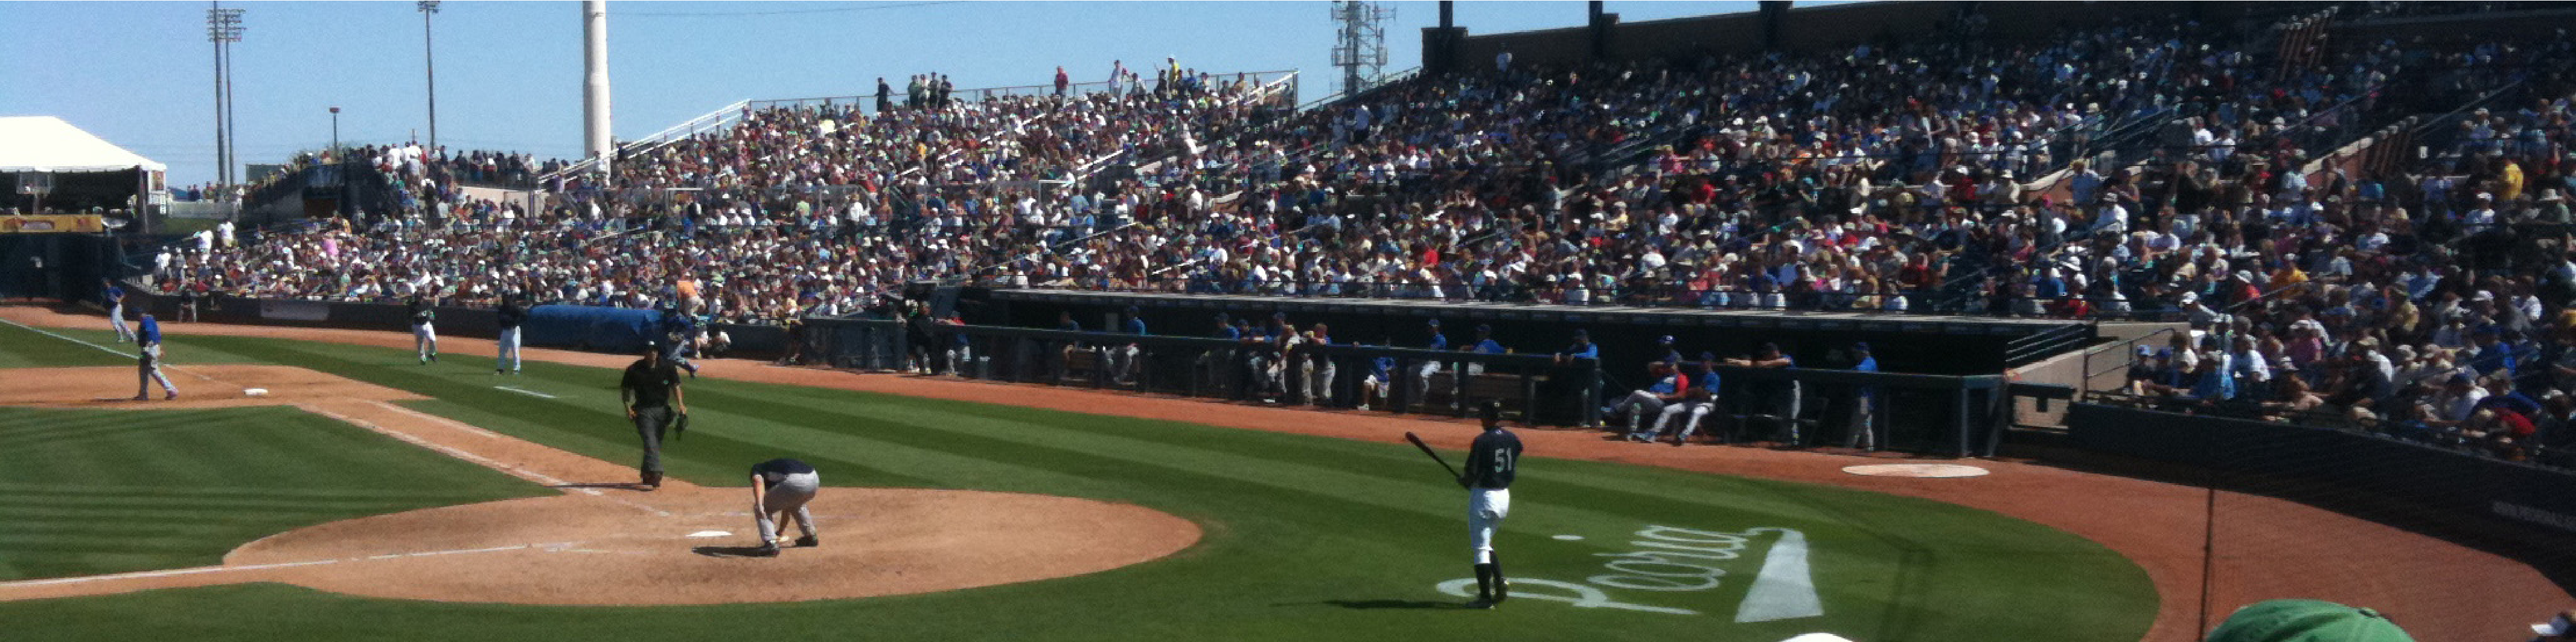
\includegraphics[width=\textwidth]{tex_sample_files/sampleteaser.pdf}
  \caption{Seattle Mariners at Spring Training, 2010.}
  \Description{Enjoying the baseball game from the third-base
  seats. Ichiro Suzuki preparing to bat.}
  \label{fig:teaser}
\end{teaserfigure}

% 4. (short) Answer Teaser
% Provides the answer on how to overcome the hurdles. Explains how this will help deflect the threats or seize the opportunities.
% keep this short
In this paper, we present a fast communication channel between a user's brain signals and a physical end effector, here EMS. Crucially, our brain-computer interface controls the user's muscles through EMS at the time of their \textit{intent to act}, as measured through readiness potentials (RP) present in the user's electroencephalogram (EEG). In our user study we applied a mixed-methods research approach to investigate whether keeping the physical impact on the user's body in line with their intention to move preserves their sense of agency.
% We found ... rendering the augmentation a \textit{natural}, integrated expansion of the user's body.

% \subsection{Preserving Agency using Brain Signals of the Intent to (Inter)act}
% 4. (long) Anwser with teaser image
% Provides the answer on how to overcome the hurdles. Explains how this will help deflect the threats or seize the opportunities.